\documentclass[12pt]{article}

\usepackage{hyperref}
\usepackage{siunitx}
\usepackage{graphicx}

\usepackage[style=ieee, backend=bibtex]{biblatex}
\renewcommand{\bibfont}{\small}
\addbibresource{notes.bib}


\title{Gazebo Motor Model Notes}

\author{Matthew Vernacchia\\
Department of Aeronautics and Astronautics, MIT}

\date{\today}


\begin{document}
\maketitle

\section{Physical Model}
Let's begin with a simple physical model of the propeller. A short introduction to propeller theory is presented in \cite{Unified}, and one can read more details in McCormick's book \cite{McCormick1979}. The model uses the following variables:

\begin{itemize}
    \item $\rho$, the air density (units: \si{\kilogram\per\meter\cubed})
    \item $T$, the thrust generated by the propeller (units: \si{\newton})
    \item $Q$, the torque generated by the propeller (units: \si{\newton\meter})
    \item $P$, the power required to drive the propeller (units: \si{\watt}).
    \item $n$, the rotation rate of the propeller (units: \si{rev \per\second}), and $\omega$, the angular speed of the propeller (units: \si{\radian\per\second}). $\omega = 2 \pi n$.
    \item $v_\parallel$ or $v_0$, the velocity at which the propeller is moving into the air along the rotation axis of the propeller (units: \si{\meter\per\second})
    \item $D$, the propeller diameter (units: \si{\meter}).
\end{itemize}

To simulate the forces and moments on a quadrotor, we need to predict how $T$ and $Q$ vary with $n$. This is acomplished using four dimensionless parameters:

\begin{itemize}
    \item $J = v_0 / D n$, the advance ratio.
    \item $C_T = T / \rho n^2 D^4$, the thrust coefficient (this is denoted as $k_T$ in \cite{Unified}).
    \item $C_Q = Q / \rho n^2 D^5$, the thrust coefficient (this is denoted as $k_Q$ in \cite{Unified}).
    \item $C_P = P / \rho n^3 D^5$, the thrust coefficient (this is denoted as $k_P$ in \cite{Unified}).
\end{itemize}

The thrust, torque, and power coefficients depend on the advance ratio $J$ and the design of the propeller\footnote{The thrust, torque and power coefficients also depend on the Reynolds and Mach number at the tip of the propeller, but for most quadrotors this is a small effect.}. To estimate the thrust and torque, we need to look up $C_T(J)$ and $C_Q(J)$ for our propeller, and then use:

\begin{equation}
    T = C_T(J) \rho n^2 D^4
\end{equation}
\begin{equation}
    Q = C_Q(J) \rho n^2 D^5
\end{equation}


The power and torque coefficients for all propellers are related by the equation $C_Q = 2 \pi C_P$. 
\[
P = Q \omega = Q (2 \pi n)
\]

\[
C_Q = \frac{Q}{\rho n^2 D^5} \left( \frac{n}{n} \right) = \frac{P}{2 \pi \rho n^3 D^5}
\]

\begin{equation}
C_Q =  \frac{C_P}{2 \pi}
\end{equation}

Most references will list only $C_T(J)$ and $C_P(J)$, but we can easliy find $C_Q$.


\section{Propellers Data}

Now we need to look up $C_T(J)$ and $C_P(J)$. UIUC provides a database of such data for small UAV/model aircraft propellers, available at \url{https://m-selig.ae.illinois.edu/props/propDB.html} \footnote{I've also incuded a zip file of the database in my repository (\url{https://github.com/mvernacc/gazebo_motor_model_docs}).}

Figure \ref{fig:prop_data_example} shows typical plots from this database. At static conditions, $C_T$ usually between $0.05$ and $0.2$, and then declines almost linearly with increasing $J$. Zero thrust usually occurs at $J = \SIrange{0.5}{1.0}{}$. $C_P$ is typically $0.03$ to $0.3$ at static conditions, and plateaus then declines with increasing $J$.

\begin{figure}
    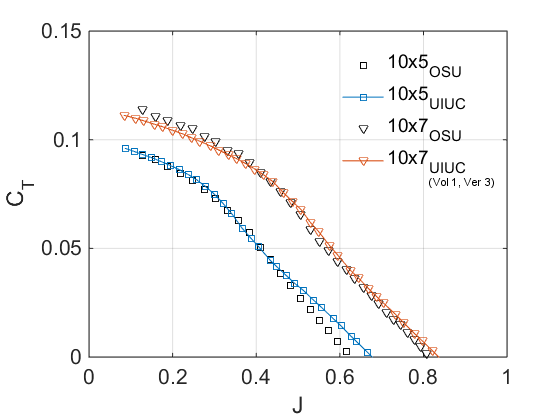
\includegraphics[width=0.5\textwidth]{UIUC-OSU-APC-E-comparison-June-2015-CT.png}
    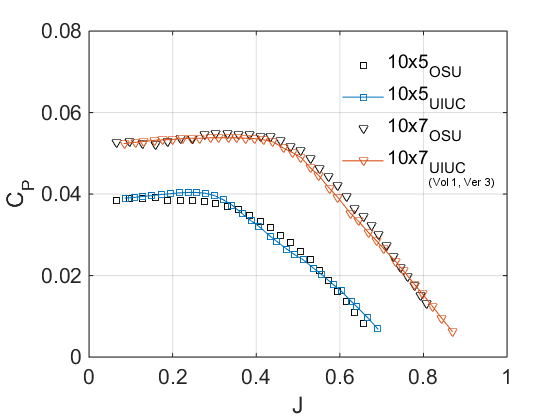
\includegraphics[width=0.5\textwidth]{UIUC-OSU-APC-E-comparison-June-2015-CP.png}
    \caption{\label{fig:prop_data_example} Example thrust and power coefficient data for two propellers (APC 10x5E and 10x7E). Reprinted from \cite{UIUCdatabase}.}
\end{figure}

In the US, propellers are designated by two numbers ``$D_{in} \times p_{in}$'', where $D_{in}$ is the diameter in inches and $p_{in}$ is the pitch in inches\footnote{The pitch angle $\beta$ is the angle bewteen the zero-lift line of the propeller blade section and the plane of rotation. The pitch $p$ is $p = \pi D \tan \beta$ for a constant-pitch propeller.} If you cannot find your vehicle's propeller in the database, use the data from a propeller design with similar ``$D_{in} \times p_{in}$''.

If no data is available, reasonable guesses for two-blade model aircraft propellers at $J=0$ (static) are $C_T = 0.1$ and $C_P = 0.05$ ($C_Q = 0.3$).

If you cannot find data for your propeller, you can also estimate the thrust and power coefficients using \emph{blade element theory}. This is rather involved. JavaProp (\url{https://www.mh-aerotools.de/airfoils/javaprop.htm}) is a free software package for perform these calculations.


\section{Current PX4 Gazebo SITL Model}

source code: \url{https://github.com/PX4/sitl_gazebo/blob/master/src/}
$gazebo_motor_model.cpp$


\section{How to Set the Parameters in the SDF}




\printbibliography

\end{document}
